% !TeX root = ../../../book.tex
\section{智力谜题}\label{sec:section1.4}

让我们将迄今为止讨论的原则付诸实践,具体研究一些有趣的数学难题及其解法。这些问题仅需基础代数与算术知识,但这绝不意味着它们``基础''或``简单'',因为解决并理解这些问题需要批判性思维与敏锐的洞察力。在此过程中,我们将运用已建立的逻辑思想,其中可能需要处理多项式函数,或用代数方法求解方程;必须仔细梳理论证的逻辑顺序,确保每一步都基于已知前提或合理推论。最重要的是,我们将思考如何构建严谨而有效的\emph{证明}来揭示数学真理!

% !TeX root = ../../../book.tex
\subsection{消失的钞票}

\subsubsection*{问题描述}

这个经典的谜题包含在一个关于分摊酒店房间费用的故事中:

\begin{quote}
    三个朋友自驾旅行,深夜入住酒店。值班店员说当晚只剩一间空房,三人合住需付 $30$ 美元。他们疲惫不堪,便同意合住,每人各付 $10$ 美元预付款。店员道谢后递过钥匙,三人随即去车上取行李。此时,前来换班的另一名店员发现前一名店员多收了房费:实际只需 $25$ 美元。于是他从收银机取出一张 $5$ 美元钞票,递给值班服务生说:``把钱退给 29 号房的客人,我们多收费了。''服务生点头后走向三人房间。客人开门时对退款又惊又喜。为公平起见,一人将钞票换成五张 $1$ 美元纸币,每人取回 $1$ 美元,剩余 $2$ 美元作为小费给了服务生。服务生道谢后离开。

    现在,三人每人实际支付 $9$ 美元房费,加上 $2$ 美元小费,总计 $29$ 美元。但他们最初支付了 $30$ 美元……消失的 $1$ 美元去哪儿了?!
\end{quote}

请仔细思考一下,然后再翻页阅读解答。

\clearpage

\subsubsection*{解答:追踪资金流向}

你搞明白了吗?其实没有任何东西凭空``消失''。这个谜题的目的就是迷惑读者,误导他们去寻找不存在的事物。题目中的数字经过精心设计,使``消失的金额''仅为 $1$ 美元,让读者误以为发生了什么神秘事件。但通过细致的逻辑分析,你会发现最终提问本身并不合理:它利用了读者对情境的误解,使其忽视逻辑推理。若数字差异变得更大,人们便不会执着于寻找``消失的钞票''。

首先,让我们分析一下在这个特殊案例中到底发生了什么。关键在于厘清资金的实际流向。我们可将参与者分为两组:朋友群体(记为 $F$)和酒店员工群体(包括店员与服务生,记为 $H$)。现在,让我们重现资金转移步骤:

\begin{enumerate}
    \item $F$ 支付 $H \quad 30$ 美元(原始房费)
    \item $H$ 退还 $F \quad \enspace 5$ 美元(多收房费退款)
    \item $F$ 支付 $H \quad \enspace 2$ 美元(服务生小费)
    \item 净变化:$F$ 向 $H$ 支付 $30 \text{\ 美元} -5 \text{\ 美元} + 2 \text{\ 美元} = 27 \text{\ 美元}$
\end{enumerate}

这样就清晰了:退款 $5$ 美元使实际房费变为 $25$ 美元,三人每人付了 $9$ 美元,再加上服务生的小费,共计 $27$ 美元。谜题错误地将小费与房费相加,但 $27$ 美元已包含全部支出。通过追踪群体间的资金流动,我们能准确还原交易过程。

\subsubsection*{泛化:改变数字}

让我们应用上述方法来修改问题,通过改变数字消除对``消失的钞票''的情感依赖,同时放大金额差异。首先定义变量表示各步骤的金额。与其``测试''特定数值,不如引入变量实现``一次性全面验证''。

设 $3n$ 表示三人首次支付的房费总额($n$ 为每人支付金额)。退款金额设为 $3r + 2$,其中 $r$ 为每人实际退款,$2$ 为给服务生的小费。下面用变量重述该问题:

\begin{quote}
    三个朋友自驾旅行,深夜入住酒店。值班店员说当晚只剩一间空房,三人合住需付 $3n$ 美元。他们疲惫不堪,便同意合住,每人各付 $n$ 美元预付款。店员道谢后递过钥匙,三人随即去车上取行李。此时,前来换班的另一名店员发现前一名店员多收了房费:实际只需 $3n - (3r + 2)$ 美元。于是他从收银机取出一张 $3r + 2$ 美元钞票,递给值班服务生说:``把钱退给 29 号房的客人,我们多收费了。''服务生点头后走向三人房间。客人开门时对退款又惊又喜。为公平起见,三人每人取回 $r$ 美元,剩余 $2$ 美元作为小费给了服务生。服务生道谢后离开。

    现在,三人每人实际支付 $n-r$ 美元房费,加上 $2$ 美元小费,总计 $3(n-r)+2$ 美元。但他们最初支付了 $3n$ 美元……消失的 $3n - [3(n - r) + 2]=3r - 2$ 美元去哪儿了?!
\end{quote}

现在问题是否更清晰了?正如我们之前解释的那样,差异源于原文将小费加入退款后的房费,再与初始 $3n$ 美元房费进行比较。正确的比较应该是,实际房费支出 $3(n-r) = 3n - 3r$,与退费后房费与小费之和 $[3n-(3r+2)] + 2 = 3n-3r$ 进行比较。两者完全相等!

\subsubsection*{泛化:留给你的问题}

谜题的原始陈述中,$n=10, r=1$,因此``消失的钞票''神奇地变为 $3r-2=1$。如果我们选择更大的数值——例如 $n=100, r=10$——那么 $300$ 美元的房间实际花费 $268$ 美元,服务生会退还三人 $32$ 美元,他们每人拿回 $10$ 美元,服务生保留 $2$ 美元,差额就变成了 $28$ 美元。真的会有人相信 $28$ 美元在此交易中凭空消失了吗?如果我们使用更大的 $n$ 和 $r$ 值呢?你能把差额扩大到多大?或缩小到多小?给定所需的差额(以美元为单位),你能找到满足条件的 $n$ 和 $r$ 的值吗?有多少种方法可以做到这一点?

\subsubsection*{解题心得}

逻辑和理性思维在解决难题时至关重要,因为情绪容易误导人。如果我们最初将这个谜题表述为``消失的 $28$ 美元'',你会有同样的反应吗?在试图回溯并弄清真相之前,你是否会感到短暂的困惑?


% !TeX root = ../../../book.tex
\subsection{高斯驾到}\label{sec:section1.4.2}

\subsubsection*{问题描述}

数学界流传着一个关于史上最伟大数学家兼物理学家之一——卡尔·弗里德里希·高斯 (Carl Friedrich Gauss) 的著名轶事。无论故事真实与否,其魅力令无数人深信不疑。高斯活跃于 18 世纪末至 19 世纪中叶,在数论、复分析、光学、几何学及天文学等诸多领域做出了奠基性贡献。请阅读下面这则故事,设想自己(无论童年或现在)会如何应对,然后再继续探讨。

\begin{quote}
    清晨,小学教室里喧闹的学生令老师不胜其烦。为获得片刻安宁,他急需让学生们专注做事。老师高声要求学生取出石板和粉笔。待众人准备就绪,他布置了一道题目:计算从 $1$ 到 $100$ 所有整数之和,并承诺最先完成者可担任当日助教。老师回到座位,料想繁重的计算将让学生们安静许久。不料仅过一分钟,一个男孩便带着写有答案的石板前来。老师惊讶之余亲自验算,结果证实男孩答案完全正确。他是如何快速完成计算的?
\end{quote}

请认真思考后再翻阅解答。请注意:这则故事``发生''在计算器尚未问世的年代,解题只能依靠纸笔与心算能力。

\clearpage

\subsubsection*{解答:简化计算}

也许你已经找到了窍门。实际上,这个问题有多种解法,它们大多基于相同的核心思路:尽量减少所需的计算量。

如果简单地遍历这 $100$ 个数字并逐个累加,需要进行 $99$ 次加法,且运算数字会越来越大。当然,技巧不仅仅在于更快地执行加法,而在于从根本上提高计算效率。我们知道,乘法本质上是数字与其自身的重复加法。因此,如果能找到合适的数字进行重复自加,就有可能将大量加法简化为一次乘法。

另一个关键点是加法满足\textbf{结合律}和\textbf{交换律},这意味着加法的顺序不影响最终结果。具体而言,无论将数字从 $1$ 加到 $100$ 还是从 $100$ 加到 $1$,其总和 $S$ 都相同。我们可以这样表示:
\begin{center}
    \begin{tabular}{ccccccccccccccc}
          1 & + &   2 & + &   3 & + & \dots & + &  98 & + &  99 & + & 100 & = & S\\\noalign{\smallskip\smallskip}
        100 & + &  99 & + &  97 & + & \dots & + &   3 & + &   2 & + &   1 & = & S\\\noalign{\smallskip\smallskip}
        \hline
        101 & + & 101 & + & 101 & + & \dots & + & 101 & + & 101 & + & 101 & = & 2S\\\noalign{\smallskip\smallskip}
    \end{tabular}
\end{center}
注意,我们以两种顺序写出了总和 $S$。将这两个等式逐项相加,得到总和 $2S$ 的表达式。这个新表达式可直接转换为乘法,因为有 $100$ 项,每项都等于 $101$。因此:
\begin{align*}
    2S &= 101 \cdot 100 \\
     S &= 101 \cdot 50 = 5050
\end{align*}
这比执行 $99$ 次加法要快得多。事实上,只要稍加练习,我们完全能在脑海中完成整个计算过程!

\subsubsection*{另一种解法:配对法}

解决该问题的相似思路是省去两行相加的中间步骤,直接将原始求和中的数字配对,如下所示:
\begin{align*}
    S &= 1 + 2 + 3 + \dots + 98 + 99 + 100 \\
    &= (1 + 100) + (2 + 99) + (3 + 98) + \dots + (49 + 52) + (50 + 51) \\
    &= 101 + 101 + \dots + 101 = 50 \cdot 101 = 5050
\end{align*}
该方法与前述解法本质相同,均利用加法交换律和结合律重组求和项,只是跳过了求 $2S$ 表达式然后再除以 $2$ 这一中间步骤。

\subsubsection*{泛化:$n$ 为偶数}

如果老师要求学生计算 $1$ 到 $1000$ 的数字之和呢?学生是否会抗议?高斯能否同样迅速作答?我们虽不确定前两个问题的答案,但相信你一定能轻松解决。这里唯一不同的是,我们需要创建 $500$ 组配对(而非 $50$ 组),每组之和为 $1001$(而非 $101$),因此结果为
\[1 + 2 + 3 + \dots + 998 + 999 + 1000 = 1001 \cdot 500 = 500500\]

看起来是不是存在某种规律呢?你觉得你能在不进行乘法的情况下立即说出 $1$ 到 $100$ 万之间所有数字之和是多少吗?

\subsubsection*{泛化:$n$ 为奇数}

如果老师要求的是前 $99$ 个数字之和呢?配对法是否仍然适用?让我们验证一下:
\begin{align*}
    S &= 1 + 2 + 3 + \dots + 97 + 98 + 99 \\
    &= (1 + 99) + (2 + 98) + (3 + 97) + \dots + (48 + 52) + (49 + 51) + 50 \\
    &= (49 \cdot 100) + 50 = 4950
\end{align*}
请注意,总项数为奇数,因此无法将所有数字完全配对,必须在乘法结果上加上中间项 $50$。是否有其他配对方式?
\begin{align*}
    S &= 1 + 2 + 3 + \dots + 97 + 98 + 99 \\
    &= (1 + 98) + (2 + 97) + (3 + 96) + \dots + (48 + 51) + (49 + 50) + 99 \\
    &= (49 \cdot 99) + 99 = 50 \cdot 99 = 4950
\end{align*}
这种方法\emph{看起来}与原始谜题的结果更相似,因为我们只执行\emph{一次}乘法。这是巧合吗?请尝试用相同方法计算其他奇数项之和:前 $7$ 个整数之和是多少?前 $29$ 个呢?前 $999$ 个呢?前 $999999$ 个呢?

\subsubsection*{泛化:任意 $n$}

让我们从个案研究中抽离出来,尝试从更一般的视角解决这个问题。假设老师向学生提出了以下问题:
\begin{quote}
    给出前 $n$ 个自然数之和的公式。我需要一个具体的公式,这样当有人告诉我 $n$ 的值时,我就能直接代入并快速得到答案。
\end{quote}

第二句的说明排除了其他方法。虽然我们之前提出过一些简单算法,但现在被要求给出一个直接计算的公式。该如何入手呢?根据之前的观察,分情况讨论 $n$ 的奇偶性是一个合理的策略。我们发现奇偶情况下的配对结果略有差异,因此先讨论其中一种情况,再讨论另一种。在每种情况下,我们都寻求 $S(n) = 1 + 2 + 3 + \dots + (n - 2) + (n - 1) + n$ 的表达式。这里用 $S(n)$ 表示这个和依赖于 $n$ 的值。

如果 $n$ 为偶数,我们可以将所有数完美配对:
\begin{align*}
    S(n) &= 1 + 2 + 3 + \dots + \Big(\frac{n}{2}-1\Big) + \frac{n}{2} + \Big(\frac{n}{2}+1\Big) + \dots + (n - 2) + (n - 1) + n\\
    &=  (1 + n) + \big(2 + (n - 1)\big) + \big(3 + (n - 2)\big) + \dots + \Big(\big(\frac{n}{2}-1\big)+\big(\frac{n}{2}+2\big)\Big) + \Big(\frac{n}{2}+\big(\frac{n}{2}+1\big)\Big) \\
    &= (n+1)\frac{n}{2} = \frac{n^2+n}{2}
\end{align*}

将已知结果的偶数(如 $n=100, 1000, 1000000$)代入公式进行验证。注意,公式中出现 $\frac{n}{2}$ 是合理的,因为 $n$ 为偶数,$\frac{n}{2}$ 必为整数。

如果 $n$ 为奇数呢?此时无法将所有数完全配对,需要巧妙处理。回想前 $99$ 项求和的方法,通过暂时忽略末项 $n$,将剩余项配对。有趣的是,每对之和恰好等于末项 $n$。让我们尝试运用此方法:
\begin{align*}
    S(n) &= 1 + 2 + 3 + \dots + \Big(\frac{n-1}{2}-1\Big) + \frac{n-1}{2} + \Big(\frac{n-1}{2}+1\Big) + \dots + (n - 2) + (n - 1) + n\\
    &=  \big(1 + (n-1)\big) + \big(2 + (n - 2)\big) + \dots + \Big(\big(\frac{n-1}{2}\big)+\big(\frac{n-1}{2}+1\big)\Big) + n \\
    &= n+n+ \dots + \Big(\frac{2n-2}{2}+1\Big) +n = (n+n+\dots+n)+n
\end{align*}

这表明每对数字之和为 $n$,即我们最初忽略的末项。现在计算配对数量:第一对是 $(1, n - 1)$,第二对是 $(2, n - 2)$,依此类推,最后一对的首项为 $\frac{n-1}{2}$。因此共有 $\frac{n-1}{2}$ 对。(注意 $n$ 为奇数保证了 $n-1$ 为偶数,故 $\frac{n-1}{2}$ 为整数。请回顾推导过程,确认每一步的有效性。)加上末项 $n$,总和可表示为:
\[S(n) = \Big(\frac{n-1}{2} + 1\Big) \cdot n = \Big(\frac{n-1}{2} + \frac{2}{2}\Big) \cdot n = \frac{n+1}{2} \cdot n = \frac{n^2+n}{2}\] 

令人惊讶的是,这与 $n$ 为偶数时得到的公式完全相同!你是否感到意外?虽然奇偶情况的解法相似,但并无明显迹象预示结果会一致。这对我们有什么启示?数学家面对这种``巧合''时,会思考是否存在\emph{更简洁}、\emph{更普适}的解法——能否用一种方法同时处理奇数和偶数\emph{两种}情况?既然结果相同,这样的方法很可能存在。请在继续阅读前先思考一下这个问题。

\subsubsection*{泛化:任意 $n$, \emph{不}分开讨论}

事实证明,我们在之前讨论这道谜题时已经暗示过另一种方法。还记得将正序求和写在一行、倒序求和写在另一行并将它们相加吗?当时处理奇偶性问题时,我们因看似步骤繁琐而避开了此法;``配对法''似乎更快捷,所以我们便采用了配对法。但若重新审视``两次相加''这一方法,会得到什么?我们会发现:
\begin{center}
    \begin{tabular}{ccccccccccc}
           1  & + &     2 & + & \dots & + & (n-1) & + &     n & = & S(n)\\\noalign{\smallskip\smallskip}
           n  & + & (n-1) & + & \dots & + &     2 & + &     1 & = & S(n)\\\noalign{\smallskip\smallskip}
        \hline
        (n+1) & + & (n+1) & + & \dots & + & (n+1) & + & (n+1) & = & 2S(n)\\\noalign{\smallskip\smallskip}
    \end{tabular}
\end{center}
此时第三行求和包含 $n$ 项,每项均为 $(n + 1)$。因此:
\begin{align*}
    2S &= (n+1) \cdot n \\
     S &= \frac{1}{2}(n+1) \cdot n = \frac{n^2+n}{2}
\end{align*}
这正是此前推导的公式,而此处的推导过程完全不依赖 $n$ 的奇偶性!(请回顾上述步骤并自行验证 $n$ 的奇偶性确实无关紧要。)

\subsubsection*{第三种解法:可视化图表}

在结束此问题之前,我们介绍一种几何解法。我们将求和 $S(n)$ 与正方形的面积关联,并将求和的各项($1, 2, 3, \dots, n - 1, n$)可视化为正方形的一部分。具体来说,考虑一个 $n \times n$ 的正方形,并将各项表示为宽度为一个单位、高度递增的矩形。见下图:

\begin{center}
    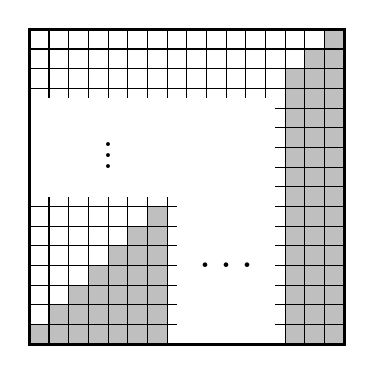
\begin{tikzpicture}[scale=0.5, x=0.5cm, y=0.5cm, font=\LARGE]
        \foreach \x in {0,...,15} 
            \foreach \y in {0,...,15}
                {
                    \pgfmathparse{(\x >= \y && (\x<7 || \x>12)) ? "lightgray" : "white"}
                    \edef\colour{\pgfmathresult}
                    \path[fill=\colour] (\x,\y) rectangle ++ (1,1);
                    \draw[black] (\x,\y) rectangle ++ (1,1);
                }
        \fill[white] (0, 7.5) rectangle ++ (8,5) node[color=black, pos=.5, align=center]{$\vdots$};
        \fill[white] (7.5, 0) rectangle ++ (5,8) node[color=black, pos=.5, align=center]{$\dots$};
        \fill[white] (7.5, 7.5) rectangle ++ (5,5) node[color=black, pos=.5, align=center]{$\iddots$};
        \draw[very thick, black] (0, 0) rectangle ++ (16,16);
    \end{tikzpicture}
\end{center}

现在,要求 $S(n)$ 的公式等价于计算正方形内所有矩形覆盖的\emph{面积}。直接相加各矩形面积只是重复原问题,因此我们需要将该面积与正方形的总面积关联。为此,考虑剩余区域,如何描述未被矩形覆盖的部分?观察第一个 $1 \times 1$ 矩形正上方的区域:它是一个尺寸为 $(n - 1) \times 1$ 的矩形。

类似地,$2 \times 1$ 矩形上方的区域是一个 $(n-2) \times 1$ 矩形。此模式持续下去!最终,在 $(n - 1) \times 1$ 矩形上方为一个 $1 \times 1$ 矩形,而最后一个 $n \times 1$ 矩形上方无区域。这些矩形的总面积类似于 $S(n)$,但缺少最后一项 $n$。现在,将所有矩形的面积与 $S(n)$ 和正方形面积关联:
\[n^2 = S(n) + (S(n) - n) = 2S(n) - n\]
解得
\[S(n) = \frac{n^2+n}{2}\]
与我们之前得到的公式一致!

\subsubsection*{解题心得}

有时,问题有多种解法。有些方法易于构思但难于求解;有些难以想到但求解简洁;还有些可能根本无效!通常无法预判哪种方法有效,因此建议动手尝试并观察结果。记录尝试的过程和结果,以便后续重新评估。这是数学学习中需牢记的原则:我们并非总能立即知晓正确路径,偶尔会陷入困境或走入死胡同。这不应令人沮丧;它是学习的一部分。

作为练习,尝试为 $n$ 为奇数的情况重新``配对'',不忽略求和的最后一项,而是分离中间项并将数字从外向内配对。这会得到相同结果吗?该方法是否比原解法更简便、更快速或有所不同呢?或者,对于 $n$ 为偶数的情况,令 $n=2k$ 会怎样?对于 $n$ 为奇数又该如何操作?这种表示会改变处理过程吗?会使问题更容易处理吗?现在,你能构思一种全新的解法吗?


% !TeX root = ../../../book.tex
\subsection{求和杂谈}\label{sec:section1.4.3}

\subsubsection*{奇数求和:观察模式}

既然谈到了整数求和,不妨探讨一些相关问题。首先介绍一种有趣的几何方法来解释奇数之和:将 $1$ 表示为 $1 \times 1$ 方块,随后每个连续的更大奇数可视作由 $1 \times 1$ 方块构成的直角,它能完美贴合前一个图形。我们为什么要这样做?因为奇数序列中连续项相差 $2$,每次将直角边增加 $1$ 个方块,即可与原图形无缝衔接,逐步构建更大的正方形!

\begin{center}
    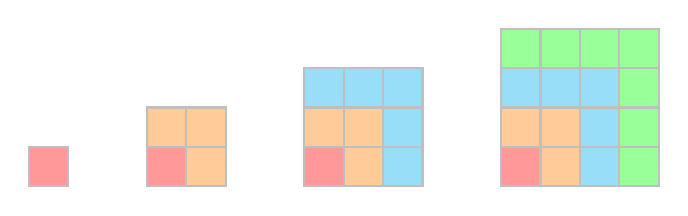
\begin{tikzpicture}[thick,scale=0.5, x=1cm, y=1cm]
        \foreach \x in {0,3,7,12}
        {
            \fill[red!40!white] (\x, 0) rectangle ++ (1,1);
            \draw[lightgray] (\x, 0) rectangle ++ (1,1);
        }

        \foreach \x in {3,7,12}
        {
            \foreach \i in {0,1}
            {
                \fill[orange!40!white] (\x+\i, 1) rectangle ++ (1,1);
                \draw[lightgray] (\x+\i, 1) rectangle ++ (1,1);
                \fill[orange!40!white] (\x+1, \i) rectangle ++ (1,1);
                \draw[lightgray] (\x+1, \i) rectangle ++ (1,1);
            }
        }

        \foreach \x in {7,12}
        {
            \foreach \i in {0,...,2}
            {
                \fill[cyan!40!white] (\x+\i, 2) rectangle ++ (1,1);
                \draw[lightgray] (\x+\i, 2) rectangle ++ (1,1);
                \fill[cyan!40!white] (\x+2, \i) rectangle ++ (1,1);
                \draw[lightgray] (\x+2, \i) rectangle ++ (1,1);
            }
        }

        \foreach \i in {0,...,3}
        {
            \fill[green!40!white] (12+\i, 3) rectangle ++ (1,1);
            \draw[lightgray] (12+\i, 3) rectangle ++ (1,1);
            \fill[green!40!white] (12+3, \i) rectangle ++ (1,1);
            \draw[lightgray] (12+3, \i) rectangle ++ (1,1);
        }
    \end{tikzpicture}
\end{center}

这种模式会持续下去吗?若确信如此,要如何严格证明?几何图案隐含的数值之和有何意义?这是首先要回答的问题,因为尽管几何呈现直观优美,但却难以精确操作和验证,最终无法给出严谨的\emph{证明}。本质上,仅展示前几项并宣称``看,它成立!''并不构成数学证明,因此需要寻求更优的表述方式。这并非否定图形的意义与美感,其运作机制确实提供了有价值的数学洞察,但归根结底,这便是其所能带给我们的上限。

\subsubsection*{奇数求和:证明我们的发现}

让我们尝试用数字形式写出上图所表示的求和。每个正方形由 $1 \times 1$ 块组成,每个比前一个多两块,因此每个正方形对应一个求和,例如
\[1 \qquad 1+3 \qquad 1+3+5 \qquad 1+3+5+7 \]
依此类推。从这些求和中,我们注意到它们都是平方数:
\[1=1^2 \qquad 1+3=4=2^2 \qquad 1+3+5=9=3^2 \qquad 1+3+5+7=16=4^2 \]
\emph{这}正是我们想要证明的模式;它对应于之前观察到的几何图形,但现在是我们可以操作的数学形式。现在,让我们思考如何证明这一点。这种模式与我们之前见过的模式相似吗?我们之前已经证明过关于整数之和的结果了吗?当然!回顾之前的题目,事实上在某些方面,我们已经证明了
\[1 + 2 + 3 + \dots + (n_1) + n =\frac{n^2 + n}{2}\]
这对该题有何用处?我们证明的求和公式涉及从 $1$ 到 $n$ 的\emph{所有}连续整数,但当前问题只考虑连续\emph{奇数}。

之前我们用函数 $S(n)$ 表示前 $n$ 个自然数之和,所以我们定义函数 $T(n)$ 表示前 $n$ 个奇数之和。首先,我们需要确定这个和的项,然后尝试将它们与 $S(n)$ 联系起来。下面,我们列出了 $n = 1, 2, 3, 4$ 时的和。你能找到一种方法来识别求和中的最大项并用 $n$ 表示它吗?
\begin{align*}
    n=1: &\quad 1\\
    n=2: &\quad 1+3\\
    n=3: &\quad 1+3+5\\
    n=4: &\quad 1+3+5+7
\end{align*}
请注意,求和项的最后一项始终为 $2n-1$。这与一般事实相关,即任何偶数都可以表示为 $2k$ 其中 $k$ 为整数,任何奇数都可以表示为 $2n - 1$,其中 $n$ 为整数。(类似地,奇数也可表示为 $2n + 1$,但这里使用 $2n - 1$ 更合适。)因此,前 $n$ 个奇数之和的公式为
\[T(n) = 1 + 3 + 5 + 7 + \dots + (2n - 3) + (2n - 1)\]
我们能否将这个求和与 $S(n)$ 或其他公式联系起来?请注意求和公式
\[S(2n) = 1 + 2 + 3 + \dots + (2n - 3) + (2n - 2) + (2n - 1) + 2n\]
包含从 $1$ 到 $2n$ 的\emph{所有}自然数,而 $T(n)$ 仅包含该范围内的奇数。或许将两个和相减,并求剩余项之和是合理的:
\begin{align*}
    S(2n) - T(n) &= 1 + 2 + 3 + \dots + (2n - 1) + 2n \\
    &\quad -\big(1 + 3 + 5 + \dots + (2n - 3) + (2n - 1)\big) \\
    & =  2 + 4 + 6 + \dots + (2n - 2) + 2n
\end{align*}
这些项都是从 $2$ 到 $2n$ 的\emph{偶数}。我们如何求得这个和?我们是否需要做额外的工作,还是可以应用之前的证明结果?由于所有项都是\emph{偶数},我们可以将所有项除以 $2$ 并写成
\begin{align*}
    \frac{1}{2}\big(S(2n) - T(n)\big) &= \frac{1}{2}\big(2 + 4 + 6 + \dots + (2n - 2) + 2n\big)\\
    &= 1 + 2 + 3 + \dots + (n - 1) + n = S(n)
\end{align*}
可以确认,最右边求和中的所有项都是整数。不仅如此,它们\emph{都是}从 $1$ 到 $n$ 的连续整数,而我们知道其求和公式!现在,所有内容都用已知公式 $S(n)$ 和 $S(2n)$ 以及所求公式 $T(n)$ 表达。最后一步是整理方程,解出 $T(n)$,并代入 $S$ 的公式:
\begin{align*}
    \frac{1}{2}\big(S(2n) - T(n)\big) &= S(n) \\
    S(2n) - T(n) &= 2S(n) \\
    T(n) &= S(2n) - 2S(n) \\
    T(n) &= \frac{(2n)^2 + 2n}{2} - \frac{2 \cdot (n^2 + n)}{2} \\
    T(n) &= \frac{4n^2 + 2n - 2n^2 - 2n}{2} \\
    T(n) &= \frac{2n^2}{2} \\ 
    T(n) &= n^2
\end{align*}
这看起来很好,不是吗?尽管需要一些代数运算,但我们得出了要证明的结论:连续奇数之和是完全平方数。不仅如此,我们还成功地精确证明了该平方数与求和项数之间的关系。具体来说,结论可简洁概括为``前 $n$ 个奇数之和等于 $n^2$''。

\subsubsection*{另一种解法:归纳证明}

我们能否用不同的方式证明这个结论?如果尚未证明上一节的结论,或者未想到那种证明方法怎么办?能否利用最初观察到的和的结构特征?

让我们换个角度思考。具体而言,探究为何在求和序列中添加一项会产生新的平方数。假设已知某个求和结果等于平方数(例如 $1 = 1^2$),现在\emph{假设}对任意项数 $n$ 均有:
\[1 + 3 + 5 + \dots + (2n - 3) + (2n - 1) = n^2\]
基于此,能否推断下一个和?添加后续奇数 $2n + 1$ 后:
\[1 + 3 + 5 + \dots + (2n - 3) + (2n - 1) + (2n + 1) = n^2 + 2n + 1 = (n + 1)^2\]
这证实了我们的推测:若前 $n$ 个奇数之和为 $n^2$,则前 $n+1$ 个奇数之和必为 $(n+1)^2$。但这是否构成完整证明?通过假设结论成立来推进证明是否合理?

这种通过已知形式推导``后续''形式的策略称为\textbf{数学归纳法}(一般来说,``后续''一词的含义取决于上下文;此处它的含义指增加求和项)。下一章将深入探讨此方法。当前需要强调的是:该策略完全有效,但高度依赖初始条件 $1 = 1^2$ 的正确性。由此可逐步推得 $1+3=2^2, 1+3+5=3^2$ 等结论。若初始条件不成立会怎样?这对归纳法有何启示?我们将在后续讨论中解决这些问题。

\subsubsection*{泛化:算术级数}

我们将探讨的最终求和问题与前两个问题密切相关。事实上,若能证明接下来的结论,就不必证明前两个结论!在这个意义上,接下来的结论更强:其真实性蕴含了前两个结论的真实性。(这是数学中常见的关系,用于描述结论之间的相对强度。)

现在,我们要为一般的\textbf{算术级数}建立一个求和公式。这意味着我们将对一个公差为固定值的级数求和,或者说,每一项由前一项加上一个固定常数得到。请注意,后两个题目中的求和对象都是算术级数:第一个求和的公差为 $1$(即每项加 $1$ 得到下一项),第二个求和的公差为 $2$(即每项加 $2$ 得到下一项)。

如何表示一个一般的算术级数?由于连续项之间相差一个固定常数,我们设此常数为 $c$。求和还需首项,设其为 $a$。此外,我们需要知道求和项数,设其为 $k$(沿用之前的变量含义)。于是,可用这三个变量表示整个求和:
\[A(a, c, k) = a + (a + c) + (a + 2c) + (a + 3c) + \dots + \big(a + (k - 2)c\big) + \big(a + (k - 1)c\big)\]
我们利用了公差为 $c$ 的性质:首项为 $a$,第二项为 $a + c$,依此类推。总项数为 $k$,首项可视为 $a + 0 \cdot c$,末项则是首项加 $k - 1$ 次 $c$ 的结果(因为从 $0$ 到 $k - 1$ 共有 $k$ 个数)。符号 $A(a, c, k)$ 表示``首项为 $a$、公差为 $c$、项数为 $k$ 的算术级数之和''。现在,如何计算这个求和?

沿用之前有效的策略:在第一个求和中,我们将级数正序与倒序相加,形成具有相同和的配对项,从而将求和转化为乘法。我们尝试将此法应用于此:
\begin{center}
    \begin{tabular}{ccccccccc}
                 a & + &      (a+c) & + & \dots & + & (a+(k-1)c) & = & A(a,c,k)\\\noalign{\smallskip\smallskip}
        (a+(k-1)c) & + & (a+(k-2)c) & + & \dots & + &          a & = & A(a,c,k)\\\noalign{\smallskip\smallskip}
        \hline
        (2a+(k-1)c)& + & (2a+(k-1)c)& + & \dots & + &(2a+(k-1)c) & = &2A(a,c,k)\\\noalign{\smallskip\smallskip}
    \end{tabular}
\end{center}
我们发现每个配对项之和均为 $2a + (k-1)c$。这样的配对项有多少?共有 $k$ 项(这正是我们选用 $k$ 的原因)。将求和表示为乘法,可得:
\[2A(a, c, k) = k \cdot (2a + (k - 1)c)\]
因此
\[A(a, c, k) = \frac{k}{2} \cdot k \cdot (2a + (k - 1)c)\]
这个结果是否符合你的预期?有时,尝试``猜测''可能的结果,再与推导结论对比,有助于理解其意义。

\subsubsection*{具体应用}

前文讨论的求和问题均为算术级数,那么该公式能否正确求解呢?第一题中取 $a = 1,c = 1, k = n$;代入公式得:
\[A(1, 1, n) = \frac{1}{2} \cdot k \cdot \big(2 + (n - 1)\big) = \frac{n}{2} \cdot(n+1) = \frac{n^2+n}{2}\]
这与我们之前的结论一致。对于第二题,变量取值如何?公式是否成立?请你自行验证结果。

\subsubsection*{另一种表示}

最后我们探讨该公式的另一种表达形式。观察括号中的项 $a + \big(a + (k-1)c\big)$,其结构是否有特殊意义?事实上,它们恰好是求和的首项与末项。因此求和公式可改写为:$A(a, c, k) = \frac{k}{2}(a + b)$,其中 $a$ 为首项,$b$ 为末项。这种形式有时更便捷。

例如求首项为 $12$、末项为 $110$、共 $14$ 项的算术级数之和,无需计算公差 $c$ 即可直接求解:$\frac{14}{2} \cdot (12 + 110) = 854$。这种方法是否更高效?此时公差 $c$ 是多少?给定 $a,b,k$ 时,是否存在快速求解 $c$ 的方法?

\subsubsection*{解题心得}

掌握已有结论有助于简化证明过程。有时虽知结论可用,却难觅应用之法。在这种情况下,我们意识到已证明的求和公式或许可以推广到其他求和,因此尝试将其应用于新问题。值得注意的是,奇数求和公式存在不依赖旧结论的独立证法。这暗示了更通用的结论——我们通过研究一般算术级数实现了这种推广。

在解决前两个求和问题时,我们采用了多种策略,但仅将其中一种策略应用于一般级数问题。这些方法能否迁移至其他场景?能否用数学归纳法证明第一个公式?能否用正序/逆序相加技术证明第二个公式?建议你尝试实践一下这些策略。这么做虽看似冗余(因为结论已知),但理解不同技术在不同情境下的应用是宝贵经验。数学证明中,策略选择往往与结论推导同等重要。因此,通过专项练习培养策略直觉,洞察其适用边界,将大有裨益。


% !TeX root = ../../../book.tex
\subsection{好友倾向}\label{sec:section1.4.4}

\subsubsection*{问题描述}

这个问题源于匈牙利社会学家的一则轶事,以及他对儿童朋友圈的观察。

\begin{quote}
    ``20 世纪 50 年代,匈牙利社会学家 S. Szalai 研究了儿童之间的友谊关系。他观察到,在任何大约 $20$ 个孩子的群体中,总能找到四个孩子,他们彼此都是朋友,或者四个孩子中没有任何两个是朋友。在得出社会学结论前,S. Szalai 咨询了三位著名的匈牙利数学家:Erdős, Turán 和 Sós。经过简短的讨论,他们表明这实际上是一种数学现象,而非社会学现象。对于至少 $18$ 个元素上的任意对称关系 $R$,存在 $4$ 个元素的子集 $S$,使得 $R$ 包含 $S$ 中的所有对,或不包含其中任何对。这一事实是 1930 年证明的拉姆齐定理 (Ramsey's theorem) 的一个特例,它奠定了拉姆齐理论 (Ramsey theory) 的基础,后来发展成为组合数学中的一个丰富领域。''\begin{flushright}——(引自麻省理工学院 Jacob Fox 教授的\href{https://math.mit.edu/~fox/MAT307-lecture01.pdf}{讲义}。)\end{flushright}
\end{quote}

现在,我们沿袭相同思路提出一个类似问题,但使用更小的数字。具体来说,我们想要找出\emph{满足}其中三人互为朋友或敌人的最小群体规模。

\begin{quote}
    假设在一群人中,任意两人要么是朋友,要么是敌人,且没有其他关系(例如没有熟人或亦敌亦友的情况)。尝试为四人群体中的每一对指定朋友或敌人关系,使得不存在三人组彼此都是朋友或全是敌人。五人群体能否实现这一条件?六人呢?七人?十人?二十人?请确定最小的群体规模,使得无论如何指定关系,都\emph{保证}存在一个三人小组,他们要么全是朋友,要么全是敌人。
\end{quote} 

请仔细思考一下,然后再翻页阅读解答。

\clearpage

\subsubsection*{有效地表述问题}

你解出来了吗?这是一个相当棘手的问题,所以即使没有得出答案也无需气馁。事实上,探究问题的过程与找到答案同等重要,因为解决路径多种多样,观察不同人如何理解这个问题总是饶有趣味。

首先,我们探讨如何清晰描述这种情境。针对此类问题,我们需要考虑一个固定规模的人群,并分析其中任意两人之间的关系。为高效验证三人子集是否满足特定性质,即是否存在三人\emph{互为}朋友或\emph{互为}敌人,必须找到一种简洁且易于阐释的关系表示方法。我们将这种三人关系称为``\textbf{同质性}''。

如何实现呢?如何表示人物及其关系?我们可以对人群编号,列出所有数对并标注 $F$(朋友)或 $E$(敌人)。以四人小组为例:
\[12F \qquad 13E \qquad 14F \qquad 23F \qquad 24E \qquad 34F\]

该群体是否满足同质性?直观验证并不容易:编号方式增加了定位三人子集的难度,且需逐一检查所有子集是否形成 $E E E$ 或 $F F F$ 关系。或许在深入解题前,我们应该寻求一种更优的信息呈现方式。能否想出更直观的方法,表示人群中每对个体的朋友或敌人关系?具体来说,我们希望通过高效手段定位三人子集,并快速识别其关系性质。

让我们尝试将每个人表示为一个点,两人间的关系用连线表示——例如蓝线代表朋友,红线代表敌人(注意:每对个体必有且仅有一种关系,故所有点之间均有彩线连接)。下图对应上述关系描述:

\begin{center}
    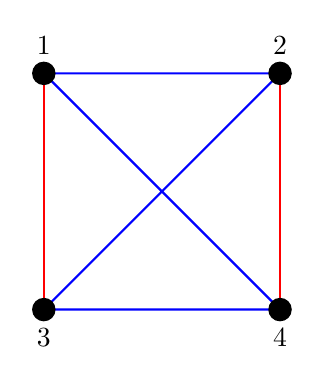
\begin{tikzpicture}[thick,scale=0.5]
        \coordinate (A) at (0,6);
        \coordinate (B) at (6,6);
        \coordinate (C) at (0,0);
        \coordinate (D) at (6,0);
        \draw[blue] (A) node[black, above, yshift=3pt]{$1$}
        -- (B) node[black, above, yshift=3pt]{$2$}
        -- (C) node[black, below, yshift=-3pt]{$3$}
        -- (D) node[black, below, yshift=-3pt]{$4$}
        -- (A);
        \draw[red] (A)--(C);
        \draw[red] (B)--(D);
        \foreach \n in {A,B,C,D}
            \node at (\n)[circle,fill,inner sep=3pt]{};
    \end{tikzpicture}
\end{center}

现在,我们要如何验证同质性?需寻找三个点(三人),其所有连线均为蓝色(全友)或红色(全敌)。这正是寻找\textbf{单色三角形}的过程!(注意:三角形顶点须为原始点,而非连线交点;术语\emph{单色 (monochromatic)} 源于希腊语 \emph{monos} 和 \emph{khroma},分别表示``一个''和``颜色''。)这种表示法更直观且便于快速检验。

根据上图,我们解决了四人问题:存在一种朋友/敌人的特定配置关系,使得其中不存在全友或全敌的三人子集。这表明四人群体可能避免同质性,故无法\emph{保证}四人中必然存在同质子集。

能否构造另一种满足该性质的配置?如何判断其与已有配置\emph{不同}?满足条件的配置共有多少种?现在请尝试构造一个\emph{必然存在}同质三人子集的配置——其形态如何?此类配置又有多少种?

\subsubsection*{重述 $n = 5$ 的问题}

让我们继续思考由五个人组成的小组。我们的图需要调整,因为现在有五个点,这意味着需要绘制更多的线。尽管如此,我们仍会用蓝色或红色线填充所有连线,并确保没有单色三角形。这可能吗?(提示:尝试将点排列成规则五边形,然后填充连线。)尝试几次,看看你的排列是否有效。随机添加几条线,并通过确保新线不会形成单色三角形来指导你的选择,这也可能有帮助。

你做出来了吗?翻页看看我们是如何做的……

\clearpage

\subsubsection*{解答:$n=5$}

这是我们在五个点之间连线的红/蓝线配置,完全避免了同质性:

\begin{center}
    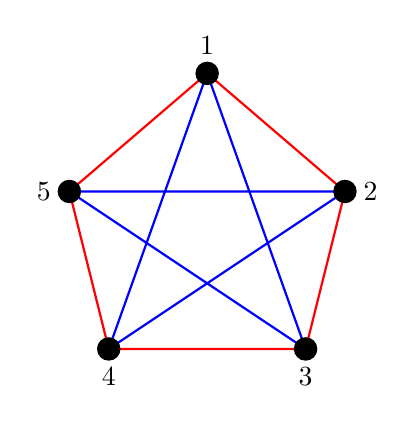
\begin{tikzpicture}[thick,scale=0.5]
        \coordinate (A) at (0,0);
        \coordinate (B) at (5,0);
        \coordinate (C) at (6,4);
        \coordinate (D) at (2.5,7);
        \coordinate (E) at (-1,4);
        \draw[red] (A) node[black, below, yshift=-3pt]{$4$}
        -- (B) node[black, below, yshift=-3pt]{$3$}
        -- (C) node[black, right, xshift=3pt]{$2$}
        -- (D) node[black, above, yshift=3pt]{$1$}
        -- (E) node[black, left, xshift=-3pt]{$5$}
        -- (A);
        \draw[blue] (A)--(D)--(B)--(E)--(C)--(A);
        \foreach \n in {A,B,C,D,E}
            \node at (\n)[circle,fill,inner sep=3pt]{};
    \end{tikzpicture}
\end{center}

请注意该图形优雅的对称性:所有红线均位于五边形的外侧,所有蓝线均位于图形内部。原因是,任意三个相邻点构成的三角形必须使用两条外线和一条内线,而任意三个不相邻点构成的三角形必须使用两条内线和一条外线。(想一想:为什么我们不能用三条内线或三条外线组成一个三角形?)这\emph{保证}了我们构成的任何三角形都会使用两种不同颜色的线,所以这个图形没有单色三角形!当然,我们可以检查图中所有可能的三角形,并确保它们都不是单色的。这样的三角形有多少个?你能多快手工找到所有这些三角形?这样做是否更容易,或者利用我们上面提到的内部/外部属性?

也许你找到的解决方案与我们的图形不同。你怎么知道它是否是不同的图形?你的图中有多少条蓝线、多少条红线?我们的图中呢?尝试通过移动点来重绘图形,但保持点之间的连接关系(即任意两点之间连线的颜色)。你能把你的图形调整得跟我们的一样吗?你认为这对本问题的解的数量意味着什么?

\subsubsection*{$n=6$ 的情况}

现在我们可以思考六个人的情况了。考虑六个点以及它们之间所有可能的连线,我们需要用蓝色或红色为每条线上色,并确保图中不存在所有边颜色相同的三角形。绘制前,请回顾四个点和五个点时我们找到的解决方案。这些解的结构如何?这次我们需要画多少条边?能否尝试构造一个与五点解相似的图形?思考当前问题与先前工作的相似之处往往大有裨益。现在,请尝试画出这个图形并观察结果。

图形是否有效?若无效,问题何在?你在何处遇到了困难?在被迫画出单色三角形之前,最多能添加多少条边?换句话说,在加入下一条必然形成单色三角形(无论颜色)的边之前,图中最多能容纳多少条边?虽然这些问题看似偏离了解决当前难题的主线,但它们本身极具启发性,并可能引导我们找到解法或其推广。为便于说明,下图展示了我们为边分配红蓝两色的一种方案。为何在此处停笔?还需添加多少条边?我们能否继续添加?

\begin{center}
    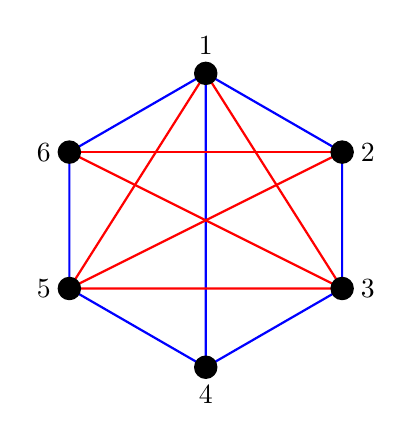
\begin{tikzpicture}[thick,scale=0.5]
        \coordinate (A) at (0,0);
        \coordinate (B) at (-3.4642,2);
        \coordinate (C) at (-3.4642,5.4642);
        \coordinate (D) at (0,7.4642);
        \coordinate (E) at (3.4642,5.4642);
        \coordinate (F) at (3.4642,2);
        \draw[blue] (A) node[black, below, yshift=-3pt]{$4$}
        -- (B) node[black, left, xshift=-3pt]{$5$}
        -- (C) node[black, left, xshift=-3pt]{$6$}
        -- (D) node[black, above, yshift=3pt]{$1$}
        -- (E) node[black, right, xshift=3pt]{$2$}
        -- (F) node[black, right, xshift=3pt]{$3$}
        -- (A)
        -- (D);
        \draw[red] (B)--(E);
        \draw[red] (C)--(F);
        \draw[red] (B)--(D)--(F)--(B);
        \draw[red] (C)--(E);
        \foreach \n in {A,B,C,D,E,F}
            \node at (\n)[circle,fill,inner sep=3pt]{};
    \end{tikzpicture}
\end{center}

我们面临的局面颇具深意,因其性质与先前情况截然相反。在四点与五点情形中,我们试图证明\emph{可以}通过边的着色方案避免单色三角形——只需构造出满足条件的\emph{具体}图形即可证明其存在性。然而对于六个点,似乎无法通过边的着色避免单色三角形。如何证明这一结论?最直接的想法是枚举所有可能的着色方案,并论证每种方案下至少存在一个单色三角形。这可行吗?着色方案共有多少种?如何在给定图形中快速定位单色三角形?回忆我们如何处理五点图形:我们注意到任何三角形必须包含\emph{至少}一条外部边与\emph{至少}一条内部边,这保证了三角形必含两种颜色的边。能否在此采用类似思路,确立某种\emph{必然}导致单色三角形存在的性质?

问题在于,六个点构成的图形中边的着色方案数量过于庞大,难以手动穷尽!图中需着色的边共有 $15$ 条,每条边可选红蓝两色,因此共有 $2^{15}$ 种着色方案——这是一个天文数字!(实际同构类会略少,因为部分方案在某种意义上是等价的;更专业地说,它们是``\emph{同构的}''。)

\subsubsection*{解答:处理\emph{任意}图形}

我们需要更巧妙的方法来论证,以便在不绘制特定图形的情况下证明\emph{任意}图形的性质。也就是说,我们需要找到对所有可能的六点图形都成立的事实,并据此推断出必然存在单色三角形。一种解决思路是关注图形的局部结构。具体而言,任取六个点中的一个,考虑从该点引出的五条边。例如,我们可能得到如下图形:

\begin{center}
    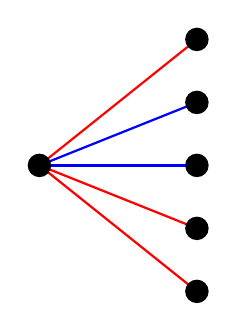
\begin{tikzpicture}[thick,scale=0.2]
        \coordinate (A) at (-6,0);
        \coordinate (B) at (4,4);
        \coordinate (C) at (4,0);
        \coordinate (D) at (4,8);
        \coordinate (E) at (4,-4);
        \coordinate (F) at (4,-8);
        \draw[blue] (A)--(C);
        \draw[blue] (A)--(B);
        \draw[red] (A)--(D);
        \draw[red] (A)--(E);
        \draw[red] (A)--(F);
        \foreach \n in {A,B,C,D,E,F}
            \node at (\n)[circle,fill,inner sep=3pt]{};
    \end{tikzpicture}
\end{center}

有多少条蓝边,多少条红边?这有些棘手:我们并非针对任何\emph{特定}图形(如上图),而是寻求适用于所有可能图形的结论。因此无法给出具体答案。面对一个\textbf{任意}图形,我们必须构建一个普遍有效的论证。

关键点在于:从该点出发的五条边中,必有三条同色(蓝或红)。试想,若非如此,则蓝边不超过两条,红边也不超过两条,总计最多四条边。但实际有五条边!(这是``\emph{抽屉原理}''的典型应用:无法将五个物体按两种颜色分类,而不使某一颜色达到三个。该原理是解决此类问题的有力工具,详见 \ref{sec:section8.6} 节。)

至此,我们得到了什么?从任意一个六点完全图中选定一点,该点必引出三条同色边。颜色可能为红或蓝,因此不能假定仅为红色;若假设为红色进行论证,之后还需讨论蓝色情况。为简化,我们首先分析从该点引出三条红边的情况(暂不限定其他边的颜色):

\begin{center}
    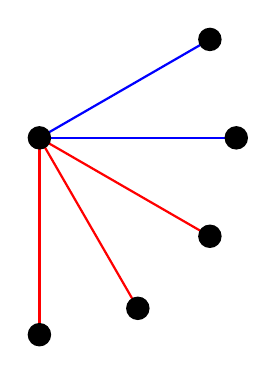
\begin{tikzpicture}[thick,scale=0.5]
        \coordinate (A) at (0,0);
        \coordinate (B) at (4.33,2.5);
        \coordinate (C) at (5,0);
        \coordinate (D) at (4.33,-2.5);
        \coordinate (E) at (2.5,-4.33);
        \coordinate (F) at (0,-5);
        \draw[blue] (A)--(C);
        \draw[blue] (A)--(B);
        \draw[red] (A)--(D);
        \draw[red] (A)--(E);
        \draw[red] (A)--(F);
        \foreach \n in {A,B,C,D,E,F}
            \node at (\n)[circle,fill,inner sep=3pt]{};
    \end{tikzpicture}
\end{center}

现在,如何添加剩余边才能避免三点间出现同色三角形?由于未限定孤立点之间边的颜色,我们聚焦于底部的三个点。它们之间的边可能是什么颜色?若其中任一条为红色,则其两个端点与原始点便构成红色三角形!这就有问题了。

\begin{center}
    \begin{tikzpicture}[thick,scale=0.5]
        \coordinate (A) at (0,0);
        \coordinate (B) at (4.33,2.5);
        \coordinate (C) at (5,0);
        \coordinate (D) at (4.33,-2.5);
        \coordinate (E) at (2.5,-4.33);
        \coordinate (F) at (0,-5);
        \draw[blue] (A)--(C);
        \draw[blue] (A)--(B);
        \draw[red] (A)--(D);
        \draw[red] (A)--(E);
        \draw[red] (A)--(F);
        \draw[red] (E)--(F);
        \draw [red,-stealth,very thick] (-2,-2.4) node[red, above]{$\text{红色三角形}$} -- (1,-3.5);
        \foreach \n in {A,B,C,D,E,F}
            \node at (\n)[circle,fill,inner sep=3pt]{};
    \end{tikzpicture}
\end{center}

避免此情况的唯一方法是将这三条边全染为蓝色。但此时,这三个点之间就形成了蓝色三角形!可见无论如何操作,都无法避免单色三角形!

\begin{center}
    \begin{tikzpicture}[thick,scale=0.5]
        \coordinate (A) at (0,0);
        \coordinate (B) at (4.33,2.5);
        \coordinate (C) at (5,0);
        \coordinate (D) at (4.33,-2.5);
        \coordinate (E) at (2.5,-4.33);
        \coordinate (F) at (0,-5);
        \draw[blue] (A)--(C);
        \draw[blue] (A)--(B);
        \draw[red] (A)--(D);
        \draw[red] (A)--(E);
        \draw[red] (A)--(F);
        \draw[blue] (F)--(D)--(E)--(F);
        \draw [blue,-stealth,very thick] (5.5,-3.8) node[blue, right]{$\text{蓝色三角形}$} -- (2.5,-3.8);
        \foreach \n in {A,B,C,D,E,F}
            \node at (\n)[circle,fill,inner sep=3pt]{};
    \end{tikzpicture}
\end{center}

现在回到抽屉原理的初始结论。若原理保证的三条同色边是蓝色而非红色呢?论证结构完全一致:观察底部三点间的边,

\begin{center}
    \begin{tikzpicture}[thick,scale=0.5]
        {
            \coordinate (A) at (0,0);
            \coordinate (B) at (4.33,2.5);
            \coordinate (C) at (5,0);
            \coordinate (D) at (4.33,-2.5);
            \coordinate (E) at (2.5,-4.33);
            \coordinate (F) at (0,-5);
            \draw[red] (A)--(C);
            \draw[red] (A)--(B);
            \draw[blue] (A)--(D);
            \draw[blue] (A)--(E);
            \draw[blue] (A)--(F);
            \draw[blue] (E)--(F);
            \draw [blue,-stealth,very thick] (-2,-2.4) node[blue, above]{$\text{蓝色三角形}$} -- (1,-3.5);
            \foreach \n in {A,B,C,D,E,F}
                \node at (\n)[circle,fill,inner sep=3pt]{};
        }
        {
            \coordinate (A1) at (8,0);
            \coordinate (B1) at (12.33,2.5);
            \coordinate (C1) at (13,0);
            \coordinate (D1) at (12.33,-2.5);
            \coordinate (E1) at (10.5,-4.33);
            \coordinate (F1) at (8,-5);
            \draw[red] (A1)--(C1);
            \draw[red] (A1)--(B1);
            \draw[blue] (A1)--(D1);
            \draw[blue] (A1)--(E1);
            \draw[blue] (A1)--(F1);
            \draw[red] (F1)--(D1)--(E1)--(F1);
            \draw [red,-stealth,very thick] (13.5,-3.8) node[red, right]{$\text{红色三角形}$} -- (10.5,-3.8);
            \foreach \n in {A1,B1,C1,D1,E1,F1}
                \node at (\n)[circle,fill,inner sep=3pt]{};
        }
    \end{tikzpicture}
\end{center}

若添加任何蓝边,会与原始点形成蓝色三角形;若全染红色,则三点间形成红色三角形!因此,无论最初的三条同色边是红色还是蓝色,论证过程完全\emph{对称}。数学家常利用这种对称性简化证明,表述为``不失一般性,假设三条边为红色''。这意味着,若选择蓝色,后续论证在数学结构上完全相同,故无需重复书写。实际上,这种情况非常常见,以至于``不失一般性''这个术语有时会缩写为 \textbf{WOLOG} 或 \textbf{WLOG} (without loss of generality)。

\subsubsection*{解答:结果总结}

截至目前我们取得了哪些进展?我们绘制了\emph{特定}图形,证明在四个或五个点之间可以着色连线而不形成单色三角形,同时推断\emph{任意}六个点构成的图形\emph{必然}包含单色三角形。对应回原始问题的朋友/敌人表述,这意味着任意六人群体中都存在一个三人组,其成员要么全部互为朋友,要么全部互为敌人。

值得注意的是,将问题转化为点线模型极具启发性;它使我们完全脱离可能分散注意力的社交背景,并简化了术语体系——将人际关系标记简化为两点间的连线。这是极具价值的解题策略:提炼问题的核心结构(底层逻辑、元素间关系及其相互作用),并据此重构表述。这种方法不仅使复杂问题更易于理解和处理,还能指导我们建立更优的符号系统。试想若坚持使用``$13F, 23E, \dots$''这类符号进行推演,也许最终也能求解,但过程必将困难重重!

原题核心目标之一是确定满足特性的最小群体规模。我们是否已完成此目标?六是否为该下界?在任意七人群体中,必然包含六人子群,而前述结论表明该子群中必定存在同质三人组(全友或全敌)。此性质自然推广至更大规模的群体,因此六确实为所求的精确下界。这与匈牙利社会学家在四人子群中观察到的现象类似,而当前问题因规模更大而显著复杂化——我们实际解决的是更小规模的简化案例。两者均属\textbf{拉姆齐理论}范畴,该组合数学与图论分支致力于探寻此类``下界规律'':当结构(如人群)规模增长至临界点时,\emph{必然}出现具备特定性质的子结构(如全友/全敌三人组)。这一始于社会现象的研究,最终被严格证明为数学定理。多么奇妙啊!

\subsubsection*{泛化:留给你的问题}

在继续之前,让我们提出一些有趣且相关的问题。如果我们要寻找不同规模的同质子群(例如四人、五人或十二人)该怎么办?一般来说,我们必须有更多的人才能保证找到这样的子群。我们能否总是这样做?也就是说,给定任何所需的子群大小,我们能否像之前那样确定一个下界?即使没有找到具体的数字,你能想出证明这种下界存在的方法吗?此外,如果我们允许第三种可能性:朋友、敌人或陌生人,又会怎样?我们能否回答关于同质子群的类似问题?这些都与拉姆齐理论相关,其中一些问题非常困难,需要数学家多年努力才能解决。许多看似简单的问题至今仍悬而未决!如果你在这些问题上没有进展,请不要灰心。我们相信,任何尝试和思考都是有意义且有益的。

\subsubsection*{解题心得}

这个问题的解决涉及几个难点。首先,我们必须找到一种方式来有效地解释谜题,以便解决问题,这涉及引入适当的符号来表示元素。这是解决数学问题的重要部分,尤其是当问题本身不提供符号或可视化时。

其次,为了确定六是群规模的下界,我们必须证明某些情况是不可能的,但可能的情况数量太多,无法逐一检验。这种情况在计算机科学和算法问题中尤其常见。为了解决这个问题,我们必须采用比大力出奇迹更巧妙的策略,但策略的选择并不总是显而易见的。在这里,我们尝试添加连接线,但最终意识到无法继续推进。证明某件事是可能的,只需提供一个例子(如我们对四人和五人组所做的那样),但证明某件事是不可能的则要复杂得多,需要针对具体情境的独创性。

最后,我们发现思考与当前问题密切相关的问题很有趣,这些问题通常只需调整原问题的一个或多个条件。如果我们寻找更大的子群怎么办?如果我们允许更多类型的连接怎么办?这将如何改变结果?通过改变这些条件来探索问题的边界,可以带来新的数学发现和技术,激励数学家积极探寻新知识并分享方法。


% !TeX root = ../../../book.tex
\subsection{三门问题}

\subsubsection*{问题描述}

这个问题仅涉及基础概率与算术,但多年来却让无数聪明人折戟沉沙。1990 年,玛丽莲·沃斯·萨万特 (Marilyn vos Savant) 在《Parade》杂志专栏发表该问题及其解法后,引发了激烈争论,许多人(包括数学家)致信赞同或反对她(正确)的答案。让我们看看你的见解!

\begin{quote}
    假设你正在参加一档游戏节目,面前有三扇门。其中一扇门后是汽车,其余两扇后是山羊。游戏开始前,汽车和山羊的位置已被随机放置在门后。游戏规则如下:你选定一扇门后,该门暂时保持关闭。主持人蒙蒂·霍尔 (Monty Hall) 知晓门后的情况,他会打开其余两扇门中有山羊的一扇。若两扇门后皆为山羊,他会随机开启一扇。蒙蒂·霍尔打开一扇有山羊的门后,会询问你:是坚持最初的选择,还是切换至另一扇关闭的门?试想:你选择了 1 号门,主持人打开了藏有山羊的 3 号门,然后问你:``是否要换到 2 号门?''改变最初的选择对你有利吗?
\end{quote}

当然,我们假设你更希望赢得汽车而非山羊,且力求最大化获胜概率。值得一提的是,该问题得名于电视节目《\emph{Let's Make a Deal}》的主持人蒙蒂·霍尔 (Monty Hall)。

那么你怎么想?试想自己站在聚光灯下,面对所有观众,当蒙蒂·霍尔问你:``要换到另一扇门吗?'' 你会作何选择?

请仔细思考一下,然后再翻页阅读解答。

\clearpage

\subsubsection*{结论:\emph{坚决}切换}

我们直接给出结论——该结论可能令人惊讶:你应当改变最初的选择!推理过程才是棘手且令人困惑的部分,而如何建立正确的解题思路正是该问题长期困扰求解者的原因。

\subsubsection*{错误论证分析}

首先展示一个常见的错误``解答'',该解答声称换门与否无关紧要。假设你与朋友讨论此题时对方提出如下解释,你会如何回应?该论证是否成立?若不同意,你会如何指出其谬误?

\begin{quote}
    当我选定一扇门后,蒙蒂·霍尔展示了另一扇有山羊的门,此时只剩两扇关闭的门。一扇后有山羊,另一扇后有汽车,因此我最初选择的门后有汽车的概率为 $50\%$,另一扇门后有汽车的概率也为 $50\%$。因此,换门不换门没有区别,还不如坚持最初的选择。
\end{quote}

上面的解释能说服你吗?让我们揭示其根本缺陷。解决此问题的关键在于计算两个概率值:坚持原选择获胜的概率,以及换门后获胜的概率。唯有准确计算并比较这两个值,才能彻底解决这个难题。

上述论证将两个概率均视为 $50\%$,但其推理存在根本缺陷。你认为坚持原选择获胜的真实概率是多少?关键在于:展示有山羊的门的行为并不会影响最初选择的门后的物体。请重点理解以下陈述:

\begin{quote}
    因为有三扇门,所以一开始选择正确的门的概率是 $\frac{1}{3}$,看到另一扇门后面有山羊\emph{并不能改变这一事实}。
\end{quote}
这正是上面错误论证的核心症结,也是``解答''本题时最常见的误区。

接下来计算换门后的胜率,并将其与 $\frac{1}{3}$ 进行比较。事实上,有多种方法可以计算此概率。一种简洁的推导是:只要初始选择的门后是山羊(概率 $\frac{2}{3}$),换门必然获胜(赢得汽车)。因为此时两扇未选门中藏着山羊与汽车,主持人必定展示有山羊的门,剩余那扇门后必定是汽车。因此换门策略的胜率为 $\frac{2}{3}$。

\subsubsection*{枚举可能性}

上述解释可能无法令你信服,我们不妨尝试实际枚举门后山羊与汽车的可能排列,并具体分析每种情况下切换选择的结果。首先请注意,门的编号并无实质影响,因为所有选择都是随机的;也就是说,无论汽车停在 1 号门、2 号门还是 3 号门后,我们最初选中汽车的概率始终是 $\frac{1}{3}$。因此可 \textbf{WOLOG}(此缩写意为``不失一般性'')假设汽车位于 1 号门后,山羊分别在 2 号门和 3 号门后。需要强调的是,这是我们自己设定的条件,参赛者并不知晓(否则必然直接选择 1 号门!)。基于此设定,我们考察初始选择的全部三种情况:

\begin{center}
    \begin{tabular}{ c|c|c } 
     1 号门 & 2 号门  & 3 号门 \\ 
     \hline 
     汽车   & 山羊    & 山羊 \\
    \end{tabular}
\end{center}

\begin{center}
    \begin{tabular}{ c|c|c|c } 
     我们的选择 & 主持人展示 & 换门结果 & 不换门结果 \\ 
     \hline 
     1 号门    & 2 号门 \:或\: 3 号门  & 山羊 & 汽车 \\
     2 号门    & 3 号门            & 汽车 & 山羊 \\
     3 号门    & 2 号门            & 汽车 & 山羊 \\
    \end{tabular}
\end{center}

关键发现在于:当我们初始选中有汽车的门时,主持人可以随机开启任意一扇有山羊的门。但无论开启哪扇门,切换选择都将失败,而坚持选择会获胜。这种情况仅占 $\frac{1}{3}$,即初始选中汽车的概率。由于表中所有情况概率均等,可以得出结论:切换策略的胜率为 $\frac{2}{3}$,而坚持策略的胜率仅为 $\frac{1}{3}$。

现在是否感觉问题更清晰了?不妨向亲友提出这个问题并观察他们的反应:有多少人答对?多少人能正确解释?多少人误答``概率相同''?又有多少人此前已经接触过此题?

\subsubsection*{泛化到多门多车情形}

让我们将这个游戏节目问题泛化,分析切换策略是否仍然有效。假设共有 $n$ 扇门和 $m$ 辆汽车,因此有 $n - m$ 只山羊。为进行有效分析,需满足 $m \le n - 2$,原因如下:

\begin{itemize}
    \item 如果 $m = n$,则无论切换与否都必然获胜,无需讨论。
    \item 如果 $m = n-1$,当初始选择有山羊的门时,主持人\emph{无法}展示另一扇有山羊的门,游戏规则无法成立,切换策略也就毫无意义。
\end{itemize}

现在,有了这些变量,游戏的新规则如下:我们随机选择一扇门。主持人从\emph{其余}门中随机打开一扇有山羊的门。此时可选择坚持最初选择或切换至\emph{任意}未打开的门。关键问题是:最优策略是什么?切换是否有利?答案是否取决于 $m$ 和 $n$?

我们将用与原题中第一种方法大致相同的方式来处理这道修改后的问题。由于 $m,n$ 为变量,我们无法枚举所有情况,只能采用逻辑推理来推断坚持和切换的胜率。首要观察与原始问题一致:\emph{坚持策略}的胜率等于初始选中汽车的概率。若初始选中有汽车的门(概率 $\frac{m}{n}$),坚持必胜;若选中有山羊的门(概率 $\frac{n-m}{n}$),坚持必败。故坚持策略的胜率为 $\frac{m}{n}$。

为了计算切换策略的胜率,需要分两种情况讨论。请注意,当 $m \geq 2$ 时,初始选中有汽车的门后切换仍可能获胜。考虑到这一点,我们需要分两种不同情况讨论:(a) 初始选中有山羊的门的情况,(b) 初始选中有汽车的门的情况。每种情况都会给主持人留下不同数量的选择,进而留下不同数量的切换策略和获胜方式,所以此处需要分开处理。

\begin{enumerate}[label=(\alph*)]
    \item \textbf{初始选中有山羊的门}。现在还剩下 $n - m - 1$ 扇有山羊的门,主持人随机选择其中一扇打开。从我们的角度来看,切换给我们留下了 $n-2$ 个选项(我们不能切换到已打开的门和最初选择的门),其中 $m$ 个是汽车。因此,在这种\emph{特定}情况下,切换后获胜的概率为 $\frac{m}{n-2}$。\\
    由于最初有 $n - m$ 只山羊,所以这种情况发生的概率为 $\frac{n-m}{n}$。因此,这种情况对切换后总获胜概率的贡献为
    \[\frac{n-m}{n} \cdot \frac{m}{n-2} = \frac{nm-m^2}{n(n-2)}\]
    (思考一下为什么我们要把这些概率相乘而不是相加?我们要如何将此概率与下一种情况的概率结合起来?)
    \item \textbf{初始选中有汽车的门}。现在还剩下 $n - m$ 扇有山羊的门,主持人随机选择其中一扇打开。从我们的角度来看,切换给我们留下了 $n-2$ 个选项,其中 $m - 1$ 个是汽车。因此,在这种\emph{特定}情况下,切换后获胜的概率为 $\frac{m-1}{n-2}$。\\
    由于最初有 $m$ 辆车,所以这种情况发生的概率为 $\frac{m}{n}$。因此,这种情况对切换后总获胜概率的贡献为
    \[\frac{m}{n} \cdot \frac{m-1}{n-2} = \frac{m^2-m}{n(n-2)}\]
\end{enumerate}

由于这两种情况是独立发生的(即它们不可能同时发生),我们需要将这两个概率相加,从而得到切换策略的总胜率:
\begin{align*}
    \frac{nm-m^2}{n(n-2)} + \frac{m^2-m}{n(n-2)} &= \frac{nm - m^2 + m^2 - m}{n(n-2)} \\
    &= \frac{nm - m}{n(n-2)} \\
    &= \frac{m(n - 1)}{n(n-2)} \\
    &= \frac{m}{n} \cdot \frac{n-1}{n-2}
\end{align*}
将此结果与坚持策略的胜率 $\frac{m}{n}$ 比较。因为 $ n - 1 > n - 2$,所以 $\frac{n-1}{n-2} > 1$,可得不等式:
\[\frac{m}{n} < \frac{m}{n} \cdot \underbrace{\frac{n-1}{n-2}}_{>1}\]
切换策略的胜率\emph{严格大于}(即总是大于)坚持策略的胜率。因此,随机切换到另一扇门总是更优策略!

\subsubsection*{具体应用}

此问题的原始版本对应 $n = 3$ 且 $m = 1$,因此可以将这些值代入来验证结果的正确性。根据推导公式,坚持策略的胜率为 $\frac{1}{3}$,而切换策略的胜率为 $\frac{1(3-1)}{3(1)} = \frac{2}{3}$,与之前的结论完全吻合!

\subsubsection*{泛化:留给你的问题}

当 $m$ 和 $n$ 取其他值时会发生什么?能否使``始终切换''策略显著优于``始终坚持''策略?两种策略的胜率差异最大能达到多少?最小又能缩小至何种程度?是否存在使两者胜率相等的情况?

该问题的另一变体是主持人开启多于一扇有山羊的门。具体设定如下:共有 $n$ 扇门,其中 $m$ 扇后有汽车;玩家首次选择后,主持人从剩余门中随机开启 $p$ 扇有山羊的门;此时玩家可选择坚持初始选择,或切换到未开启的 $n-p-1$ 扇门中的任意一扇。在此情形下最优策略是什么?需对 $m,n,p$ 施加何种约束条件以保证游戏成立?最优策略是始终切换,还是取决于 $p$ 的取值?``始终切换''与``始终坚持''策略的胜率差异范围如何?

\subsubsection*{解题心得}

直觉和快速决策有时能\emph{引导}我们找到正确答案,但务必检查这些仓促判断是否基于合理的逻辑。本题中,``$50/50$''的概率初看似乎成立,但仔细推敲后便发现其论证存在缺陷——关键在于正确解读题目并严格遵循游戏步骤的顺序。概率分析应按照游戏实际发生的流程进行,而非从结果倒推。

概率问题往往极具迷惑性,需格外审慎对待。这也揭示了一个深刻启示:看似简单的问题往往最难攻克。切勿因表述简短或易于理解而轻视问题的复杂性!

关于蒙蒂·霍尔问题及其心理学背景,请参见 \href{http://www.usd.edu/~xtwang/Papers/MontyHallPaper.pdf}{Krauss, Stefan and Wang, X. T. (2003). ``The Psychology of the Monty Hall Problem: Discovering Psychological Mechanisms for Solving a Tenacious Brain Teaser'', \emph{Journal of Experimental Psychology}: General 132(1)}。